\begin{frame}
    \frametitle{Paketa amsmath in amsfonts}
\end{frame}

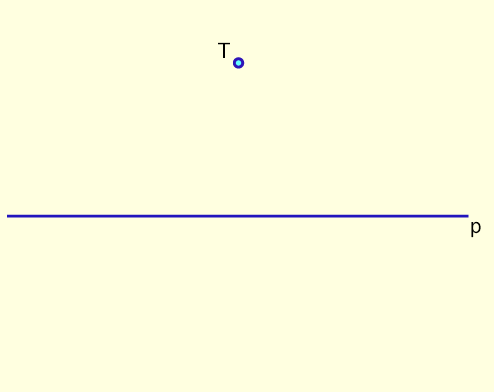
\includegraphics[width=50mm]{prosojnice/fig-1.png}
\begin{itemize}[<+->]
    \item<4>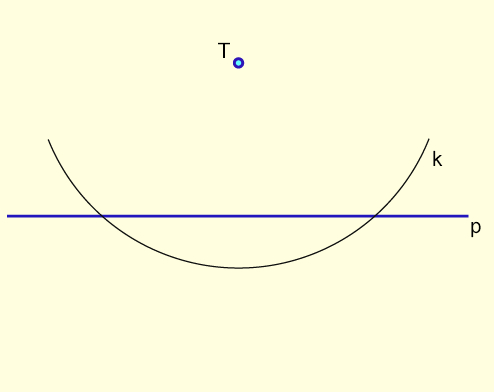
\includegraphics[width=50mm]{prosojnice/fig-2.png}
    \item Nariši lok $k$ s središčem v $T$.
    \item Premico $p$ seče v točkah $A$ in $B$.
    \item Nariši lok $m$ s središčem v $A$.
    \item Nariši lok $n$ s središčem v $B$ in z enakim polmerom.
    \item Loka se sečeta v točki $C$.
    \item Premica skozi točki $T$ in $C$ je pravokotna na $p$.
 \end{itemize}

 Dani sta premica $p$ in točka $T$.